\documentclass{article}\usepackage[]{graphicx}\usepackage[]{color}
%% maxwidth is the original width if it is less than linewidth
%% otherwise use linewidth (to make sure the graphics do not exceed the margin)
\makeatletter
\def\maxwidth{ %
  \ifdim\Gin@nat@width>\linewidth
    \linewidth
  \else
    \Gin@nat@width
  \fi
}
\makeatother

\definecolor{fgcolor}{rgb}{0.345, 0.345, 0.345}
\newcommand{\hlnum}[1]{\textcolor[rgb]{0.686,0.059,0.569}{#1}}%
\newcommand{\hlstr}[1]{\textcolor[rgb]{0.192,0.494,0.8}{#1}}%
\newcommand{\hlcom}[1]{\textcolor[rgb]{0.678,0.584,0.686}{\textit{#1}}}%
\newcommand{\hlopt}[1]{\textcolor[rgb]{0,0,0}{#1}}%
\newcommand{\hlstd}[1]{\textcolor[rgb]{0.345,0.345,0.345}{#1}}%
\newcommand{\hlkwa}[1]{\textcolor[rgb]{0.161,0.373,0.58}{\textbf{#1}}}%
\newcommand{\hlkwb}[1]{\textcolor[rgb]{0.69,0.353,0.396}{#1}}%
\newcommand{\hlkwc}[1]{\textcolor[rgb]{0.333,0.667,0.333}{#1}}%
\newcommand{\hlkwd}[1]{\textcolor[rgb]{0.737,0.353,0.396}{\textbf{#1}}}%

\usepackage{framed}
\makeatletter
\newenvironment{kframe}{%
 \def\at@end@of@kframe{}%
 \ifinner\ifhmode%
  \def\at@end@of@kframe{\end{minipage}}%
  \begin{minipage}{\columnwidth}%
 \fi\fi%
 \def\FrameCommand##1{\hskip\@totalleftmargin \hskip-\fboxsep
 \colorbox{shadecolor}{##1}\hskip-\fboxsep
     % There is no \\@totalrightmargin, so:
     \hskip-\linewidth \hskip-\@totalleftmargin \hskip\columnwidth}%
 \MakeFramed {\advance\hsize-\width
   \@totalleftmargin\z@ \linewidth\hsize
   \@setminipage}}%
 {\par\unskip\endMakeFramed%
 \at@end@of@kframe}
\makeatother

\definecolor{shadecolor}{rgb}{.97, .97, .97}
\definecolor{messagecolor}{rgb}{0, 0, 0}
\definecolor{warningcolor}{rgb}{1, 0, 1}
\definecolor{errorcolor}{rgb}{1, 0, 0}
\newenvironment{knitrout}{}{} % an empty environment to be redefined in TeX

\usepackage{alltt}

\usepackage{amsmath, amssymb}
\usepackage{graphicx}
\usepackage{hyperref}
\IfFileExists{upquote.sty}{\usepackage{upquote}}{}
\begin{document}

\title{Pol Sci 630:  Problem Set 12 Solutions: Heteroskedasticity, Autocorrelation}

\author{Prepared by: Anh Le (\href{mailto:anh.le@duke.edu}{anh.le@duke.edu})}

\date{Due Date: Friday, Nov 20, 2015, 12 AM (Beginning of Lab)}

\maketitle

\begin{knitrout}
\definecolor{shadecolor}{rgb}{0.969, 0.969, 0.969}\color{fgcolor}\begin{kframe}
\begin{alltt}
\hlkwd{rm}\hlstd{(}\hlkwc{list} \hlstd{=} \hlkwd{ls}\hlstd{())}
\hlkwd{library}\hlstd{(ggplot2)}
\end{alltt}
\end{kframe}
\end{knitrout}


\section{Heteroskedasticity}

One common cause of heteroskedasticity is that our model does not take into account heterogenous effect across sub-populations. For example, we have a model of spending (dependent var) as a function of income (independent var), and the propensity to spend differs across ethnic groups. Formally,

\begin{align}
spending &= \beta_{ethnic} income + \epsilon
\end{align}

where $\beta{ethnic}$ takes a different value for white, black, and asian. If we don't know about this heterogeneity of propensity to spend across ethnic groups, the graph will show heteroskedasticity:

\begin{knitrout}
\definecolor{shadecolor}{rgb}{0.969, 0.969, 0.969}\color{fgcolor}
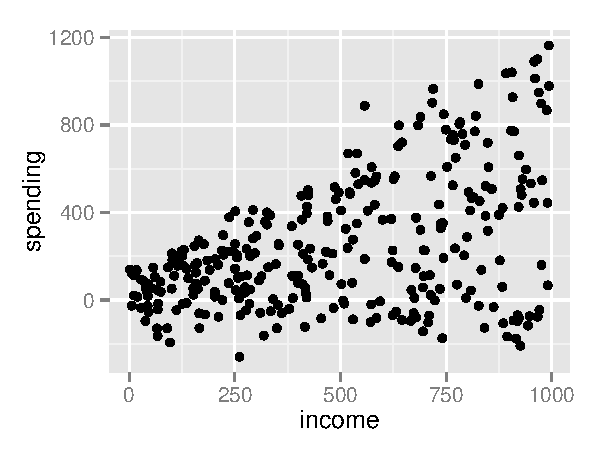
\includegraphics[width=\maxwidth]{figure/unnamed-chunk-2-1} 

\end{knitrout}

Buf if we are smart researcher, we'll realize the underlying cause of the heterogeneity, as shown in the following plot:

\begin{knitrout}
\definecolor{shadecolor}{rgb}{0.969, 0.969, 0.969}\color{fgcolor}
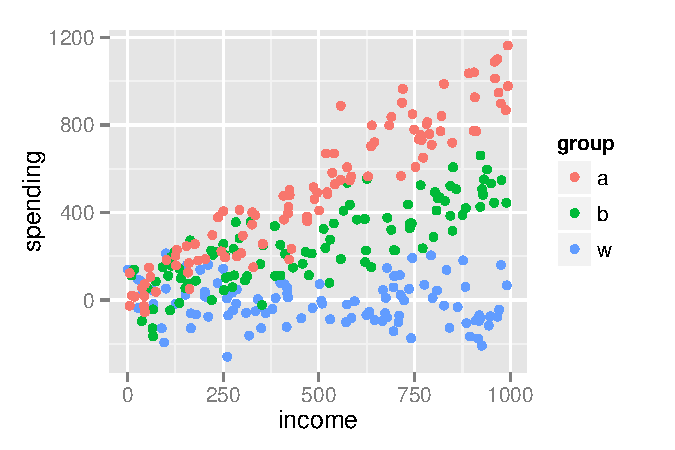
\includegraphics[width=\maxwidth]{figure/unnamed-chunk-3-1} 

\end{knitrout}

The take-home point is that heteroskedasticity could be a signal of underlying model specification, and we should think hard about the cause of heteroskedasticity instead of applying a quick fix.

\subsection{Simulating}

Simulate the spending and income pattern for three ethnic groups as described above. Re-create the two plots above. The numbers don't have to be the same -- just make sure that your data has heteroskedasticity due to underlying heterogenous effect across ethnic groups as described in the example above. Note: Don't look at my code.

\subsection{Diagnostics: Visual}

Using the simulated data above, regress spending on income, plot the residual against the predicted value.

\textbf{Solution}

\begin{knitrout}
\definecolor{shadecolor}{rgb}{0.969, 0.969, 0.969}\color{fgcolor}\begin{kframe}
\begin{alltt}
\hlstd{m_het} \hlkwb{<-} \hlkwd{lm}\hlstd{(spending} \hlopt{~} \hlstd{income,} \hlkwc{data} \hlstd{= d)}
\hlkwd{plot}\hlstd{(}\hlkwd{predict}\hlstd{(m_het),} \hlkwd{resid}\hlstd{(m_het))}
\end{alltt}
\end{kframe}
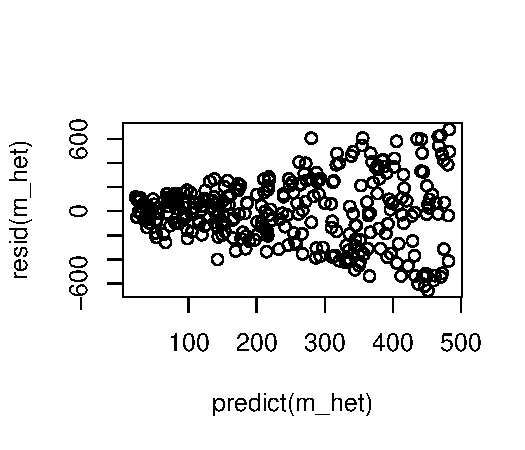
\includegraphics[width=\maxwidth]{figure/unnamed-chunk-4-1} 

\end{knitrout}

\subsection{Diagonistics: Hypothesis test}

Conduct BP test and White test. Why do the tests reach the same conclusion here, unlike in the lab tutorial?

\textbf{Solution}

\begin{knitrout}
\definecolor{shadecolor}{rgb}{0.969, 0.969, 0.969}\color{fgcolor}\begin{kframe}
\begin{alltt}
\hlkwd{library}\hlstd{(AER)}
\hlkwd{bptest}\hlstd{(m_het,} \hlkwc{varformula} \hlstd{=} \hlopt{~} \hlstd{d}\hlopt{$}\hlstd{income)}
\end{alltt}
\begin{verbatim}
## 
## 	studentized Breusch-Pagan test
## 
## data:  m_het
## BP = 98.029, df = 1, p-value < 2.2e-16
\end{verbatim}
\begin{alltt}
\hlkwd{bptest}\hlstd{(m_het,} \hlkwc{varformula} \hlstd{=} \hlopt{~} \hlstd{d}\hlopt{$}\hlstd{income} \hlopt{+} \hlkwd{I}\hlstd{(d}\hlopt{$}\hlstd{income}\hlopt{^}\hlnum{2}\hlstd{))}
\end{alltt}
\begin{verbatim}
## 
## 	studentized Breusch-Pagan test
## 
## data:  m_het
## BP = 104.89, df = 2, p-value < 2.2e-16
\end{verbatim}
\end{kframe}
\end{knitrout}

The test reaches the same conclusion because the variance of the error terms is a linear function of $income$ (not of $income^2$, for example), so both the BP and the White tests are able to detect this.

\subsection{Fixing: robust standard error}

Run hypothesis test without and with robust standard error. What's the conclusion?

\textbf{Solution}

\begin{knitrout}
\definecolor{shadecolor}{rgb}{0.969, 0.969, 0.969}\color{fgcolor}\begin{kframe}
\begin{alltt}
\hlkwd{summary}\hlstd{(m_het)}
\end{alltt}
\begin{verbatim}
## 
## Call:
## lm(formula = spending ~ income, data = d)
## 
## Residuals:
##    Min     1Q Median     3Q    Max 
## -660.3 -175.0    6.6  149.0  680.3 
## 
## Coefficients:
##             Estimate Std. Error t value Pr(>|t|)    
## (Intercept) 21.22530   30.19268   0.703    0.483    
## income       0.46486    0.05246   8.860   <2e-16 ***
## ---
## Signif. codes:  0 '***' 0.001 '**' 0.01 '*' 0.05 '.' 0.1 ' ' 1
## 
## Residual standard error: 269 on 298 degrees of freedom
## Multiple R-squared:  0.2085,	Adjusted R-squared:  0.2059 
## F-statistic: 78.51 on 1 and 298 DF,  p-value: < 2.2e-16
\end{verbatim}
\begin{alltt}
\hlkwd{coeftest}\hlstd{(m_het,} \hlkwc{vcov} \hlstd{=} \hlkwd{vcovHC}\hlstd{(m_het,} \hlkwc{type} \hlstd{=} \hlstr{"HC"}\hlstd{))}
\end{alltt}
\begin{verbatim}
## 
## t test of coefficients:
## 
##              Estimate Std. Error t value  Pr(>|t|)    
## (Intercept) 21.225300  20.346658  1.0432    0.2977    
## income       0.464863   0.057242  8.1210 1.236e-14 ***
## ---
## Signif. codes:  0 '***' 0.001 '**' 0.01 '*' 0.05 '.' 0.1 ' ' 1
\end{verbatim}
\end{kframe}
\end{knitrout}

Both regressions show that income has a positive and significant impact on spending

\subsection{Fixing: FGLS}

Conduct FGLS. Hint: For stability, log transform $residual^2$ in the auxiliary regression, then exponentiate the predicted value of the auxiliary regression to get the weight.

\textbf{Solution}

\begin{knitrout}
\definecolor{shadecolor}{rgb}{0.969, 0.969, 0.969}\color{fgcolor}\begin{kframe}
\begin{alltt}
\hlstd{auxiliary_FGLS} \hlkwb{<-} \hlkwd{lm}\hlstd{(}\hlkwd{I}\hlstd{(}\hlkwd{log}\hlstd{(}\hlkwd{resid}\hlstd{(m_het)}\hlopt{^}\hlnum{2}\hlstd{))} \hlopt{~} \hlstd{d}\hlopt{$}\hlstd{income)}
\hlstd{w} \hlkwb{<-} \hlkwd{exp}\hlstd{(}\hlkwd{predict}\hlstd{(auxiliary_FGLS))}
\hlstd{m_het_wls} \hlkwb{<-} \hlkwd{lm}\hlstd{(spending} \hlopt{~} \hlstd{income,} \hlkwc{weights} \hlstd{=} \hlnum{1} \hlopt{/} \hlstd{w,} \hlkwc{data} \hlstd{= d)}
\hlkwd{summary}\hlstd{(m_het_wls)}
\end{alltt}
\begin{verbatim}
## 
## Call:
## lm(formula = spending ~ income, data = d, weights = 1/w)
## 
## Weighted Residuals:
##     Min      1Q  Median      3Q     Max 
## -4.4095 -1.3527  0.0594  1.4140  4.0674 
## 
## Coefficients:
##             Estimate Std. Error t value Pr(>|t|)    
## (Intercept) 24.35206   15.11258   1.611    0.108    
## income       0.45591    0.04491  10.152   <2e-16 ***
## ---
## Signif. codes:  0 '***' 0.001 '**' 0.01 '*' 0.05 '.' 0.1 ' ' 1
## 
## Residual standard error: 1.621 on 298 degrees of freedom
## Multiple R-squared:  0.257,	Adjusted R-squared:  0.2545 
## F-statistic: 103.1 on 1 and 298 DF,  p-value: < 2.2e-16
\end{verbatim}
\end{kframe}
\end{knitrout}

FGLS also confirms that income has a positive and significant impact on spending.

\subsection{Fixing: Provide a correct model}

Specify a regression model that takes into account heterogenous effect of income on spending across ethnic groups. Show that there's no longer heteroskedasticity.

\textbf{Solution}

\begin{knitrout}
\definecolor{shadecolor}{rgb}{0.969, 0.969, 0.969}\color{fgcolor}\begin{kframe}
\begin{alltt}
\hlstd{m_group} \hlkwb{<-} \hlkwd{lm}\hlstd{(spending} \hlopt{~} \hlstd{income} \hlopt{+} \hlstd{group} \hlopt{+} \hlstd{income}\hlopt{:}\hlstd{group,} \hlkwc{data} \hlstd{= d)}
\hlkwd{plot}\hlstd{(}\hlkwd{resid}\hlstd{(m_group)} \hlopt{~} \hlkwd{predict}\hlstd{(m_group))}
\end{alltt}
\end{kframe}
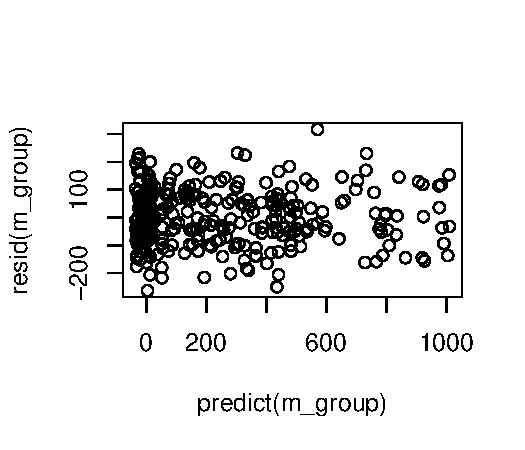
\includegraphics[width=\maxwidth]{figure/unnamed-chunk-8-1} 

\end{knitrout}

As shown in the diagnostics plot, there's no longer heteroskedasticity

\section{Multicollinearity}

\subsection{Diagnosing with VIF}

Using dataset \verb`Prestige`, run regression of prestiage against income, education, and women. Calculate VIF. Interpret the largest VIF.

\textbf{Solution}

\begin{knitrout}
\definecolor{shadecolor}{rgb}{0.969, 0.969, 0.969}\color{fgcolor}\begin{kframe}
\begin{alltt}
\hlkwd{vif}\hlstd{(}\hlkwd{lm}\hlstd{(prestige} \hlopt{~} \hlstd{income} \hlopt{+} \hlstd{education} \hlopt{+} \hlstd{women,} \hlkwc{data}\hlstd{=Prestige))}
\end{alltt}
\begin{verbatim}
##    income education     women 
##  2.282038  1.845165  1.526593
\end{verbatim}
\end{kframe}
\end{knitrout}

The largest VIF is 2.28 for income, meaning that by including other variables, the variance of the coefficient for income is inflated 2.28 times.

\subsection{Dealing with multicollinearity}

If you are concerned that the VIF is causing your SEs to be pretty big. What should you do to address this issue?

\textbf{Solution}

\textit{Note to grader: Just grade on how the submission makes an argument. We don't expect everyone to hit all the points below.}

We should either collect more data (and hopefully the multicollinearity only exists in the previous sample and not in population), or to live with imprecision in our estimates, as omitting variables would likely lead to OVB.

It's important to note that there's no magic statistical fix for multicollinearity. If two variables are highly correlated, it's simply impossible to vary one and control for the other.

One thing one may do is to conduct dimension reduction (e.g. factor analysis, PCA) so that we recover the latent factor that drives all of these highly correlated variables. For example, in a survey of governance, we may see that the measurement of road quality, electricity quality, water quality are all highly correlated. Perhaps there's a common and latent factor of ``public provision'' that drives all of them.


\section{Diagnosing autocorrelation}

\subsection{Generating autocorrelated data}

Similar to the lab, generate data (i.e. e, X, Y) that follow an AR(2) process, i.e.:

\begin{align}
v(t) &\sim N(0, 1) \\
e(t) &= a_1e(t-1) + a_2 e(t-2) + v(t) \qquad \text{Important: $a_1 + a_2 < 1$} \\
Y(t) &= X(t) + e(t)
\end{align}

\textbf{Solution}

\begin{knitrout}
\definecolor{shadecolor}{rgb}{0.969, 0.969, 0.969}\color{fgcolor}\begin{kframe}
\begin{alltt}
\hlstd{T} \hlkwb{<-} \hlnum{100} \hlcom{# Num of time periods}

\hlcom{# Generate autocorrelated e}
\hlstd{e} \hlkwb{<-} \hlkwd{vector}\hlstd{(}\hlkwc{mode} \hlstd{=} \hlstr{'numeric'}\hlstd{,} \hlkwc{length} \hlstd{= T)}
\hlstd{e[}\hlnum{1}\hlstd{]} \hlkwb{<-} \hlkwd{rnorm}\hlstd{(}\hlnum{1}\hlstd{)}
\hlstd{e[}\hlnum{2}\hlstd{]} \hlkwb{<-} \hlnum{0.4} \hlopt{*} \hlstd{e[}\hlnum{1}\hlstd{]} \hlopt{+} \hlkwd{rnorm}\hlstd{(}\hlnum{1}\hlstd{)}
\hlkwa{for} \hlstd{(t} \hlkwa{in} \hlnum{3}\hlopt{:}\hlstd{T) \{}
  \hlstd{e[t]} \hlkwb{<-} \hlnum{0.4} \hlopt{*} \hlstd{e[t} \hlopt{-} \hlnum{1}\hlstd{]} \hlopt{+} \hlnum{0.2} \hlopt{*} \hlstd{e[t} \hlopt{-} \hlnum{2}\hlstd{]} \hlopt{+} \hlkwd{rnorm}\hlstd{(}\hlnum{1}\hlstd{)}
\hlstd{\}}

\hlstd{X} \hlkwb{<-} \hlkwd{rnorm}\hlstd{(T)}
\hlstd{Y} \hlkwb{<-} \hlstd{X} \hlopt{+} \hlstd{e}
\end{alltt}
\end{kframe}
\end{knitrout}

\subsection{Diagnostics: Visual}

Plot residual against time and against lagged , up to 4 lags (e.g. residual ~ lag-1 residual, residual ~ lag-2 residual, etc. up to 4 plots) How does the correlation look across the four plots?

\textbf{Solution}

\begin{knitrout}
\definecolor{shadecolor}{rgb}{0.969, 0.969, 0.969}\color{fgcolor}\begin{kframe}
\begin{alltt}
\hlstd{lag} \hlkwb{<-} \hlkwa{function}\hlstd{(}\hlkwc{x}\hlstd{,} \hlkwc{lag_period}\hlstd{) \{}
  \hlkwd{return}\hlstd{(}\hlkwd{c}\hlstd{(}\hlkwd{rep}\hlstd{(}\hlnum{NA}\hlstd{, lag_period), x[}\hlnum{1}\hlopt{:}\hlstd{(}\hlkwd{length}\hlstd{(x)} \hlopt{-} \hlstd{lag_period)]))}
\hlstd{\}}

\hlstd{m_auto} \hlkwb{<-} \hlkwd{lm}\hlstd{(Y} \hlopt{~} \hlstd{X)}
\hlstd{e} \hlkwb{<-} \hlkwd{resid}\hlstd{(m_auto)}

\hlkwd{par}\hlstd{(}\hlkwc{mfrow} \hlstd{=} \hlkwd{c}\hlstd{(}\hlnum{2}\hlstd{,} \hlnum{2}\hlstd{))}
\hlkwd{plot}\hlstd{(}\hlkwd{lag}\hlstd{(e,} \hlnum{1}\hlstd{), e)}
\hlkwd{plot}\hlstd{(}\hlkwd{lag}\hlstd{(e,} \hlnum{2}\hlstd{), e)}
\hlkwd{plot}\hlstd{(}\hlkwd{lag}\hlstd{(e,} \hlnum{3}\hlstd{), e)}
\hlkwd{plot}\hlstd{(}\hlkwd{lag}\hlstd{(e,} \hlnum{4}\hlstd{), e)}
\end{alltt}
\end{kframe}
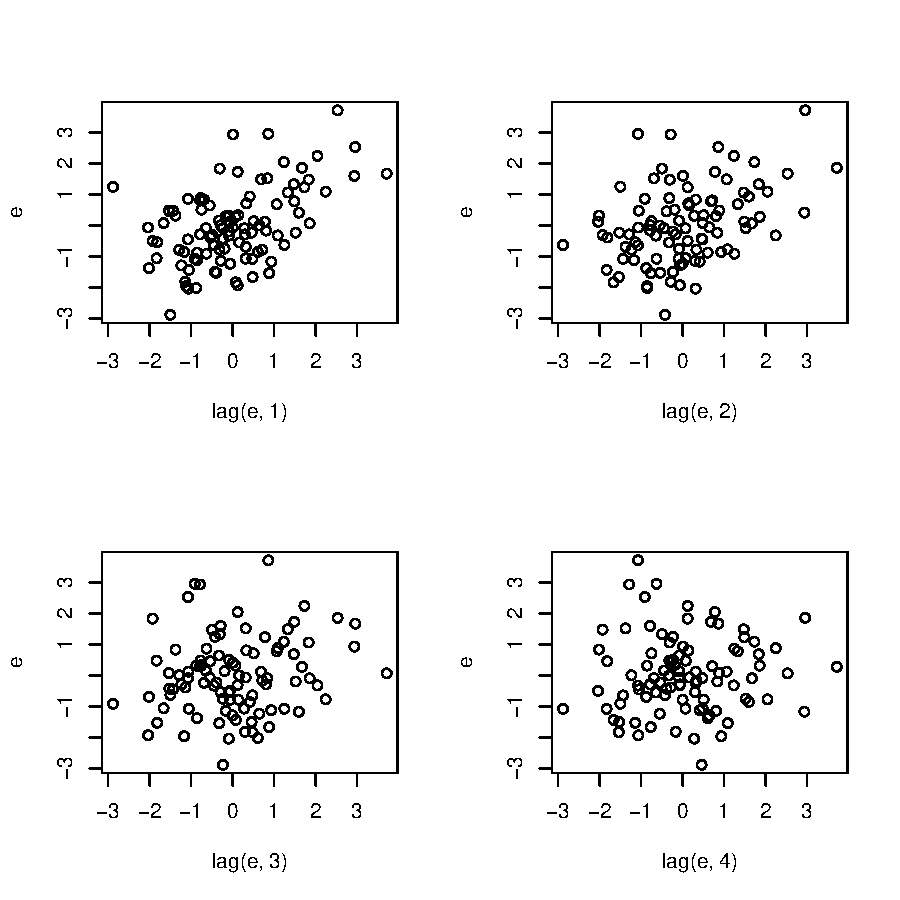
\includegraphics[width=\maxwidth]{figure/unnamed-chunk-11-1} 

\end{knitrout}

We see that he error autocorrelation diminishes the further the lag is (See how the relationship is very strong in the first plot, but not so much in the fourth?).

\subsection{Diagnostics: Hypothesis testing}

Regress residuals against X and lag1 and lag2 residuals, and then doing an F test for joint significance in the lagged residuals.

\textbf{Solution}

\begin{knitrout}
\definecolor{shadecolor}{rgb}{0.969, 0.969, 0.969}\color{fgcolor}\begin{kframe}
\begin{alltt}
\hlstd{lag1_e} \hlkwb{<-} \hlkwd{lag}\hlstd{(e,} \hlnum{1}\hlstd{)}
\hlstd{lag2_e} \hlkwb{<-} \hlkwd{lag}\hlstd{(e,} \hlnum{2}\hlstd{)}

\hlcom{# Reg residual against X and lagged residuals}
\hlstd{m_autotest} \hlkwb{<-} \hlkwd{lm}\hlstd{(e} \hlopt{~} \hlstd{X} \hlopt{+} \hlstd{lag1_e} \hlopt{+} \hlstd{lag2_e)}

\hlcom{# Doing an F test}
\hlkwd{library}\hlstd{(car)} \hlcom{# to run F-test}
\hlkwd{linearHypothesis}\hlstd{(m_autotest,} \hlkwd{c}\hlstd{(}\hlstr{"lag1_e"}\hlstd{,} \hlstr{"lag2_e"}\hlstd{))}
\end{alltt}
\begin{verbatim}
## Linear hypothesis test
## 
## Hypothesis:
## lag1_e = 0
## lag2_e = 0
## 
## Model 1: restricted model
## Model 2: e ~ X + lag1_e + lag2_e
## 
##   Res.Df    RSS Df Sum of Sq      F   Pr(>F)    
## 1     96 147.25                                 
## 2     94 105.30  2    41.952 18.725 1.43e-07 ***
## ---
## Signif. codes:  0 '***' 0.001 '**' 0.01 '*' 0.05 '.' 0.1 ' ' 1
\end{verbatim}
\end{kframe}
\end{knitrout}

We reject the null of no autocorrelation. Notice how we can do the F-test on more than just one lag to detect autocorrelation. In real research, you would use your judgement to guess the autocorrelation structure (i.e. how far back does the autocorrelation go?) and test it.

\end{document}
